%\chapter{Decomposition view (UML Component diagram)}\label{ch:decomposition}

% Delete the command below to remove the hints and instructions
\showdecompnotes{}

% \begin{figure}[!htp]
% 	\centering
% 	%\includegraphics[width=\textwidth]{}
% 	\missingfigure[figwidth=0.8\textwidth]{Diagram showing decomposition of ComponentX}
% 	\caption{Decomposition of \texttt{ComponentX}}\label{fig:decomp-componentx}
% \end{figure}

\begin{landscape}
    \begin{figure}[!htp]
    	\centering
    	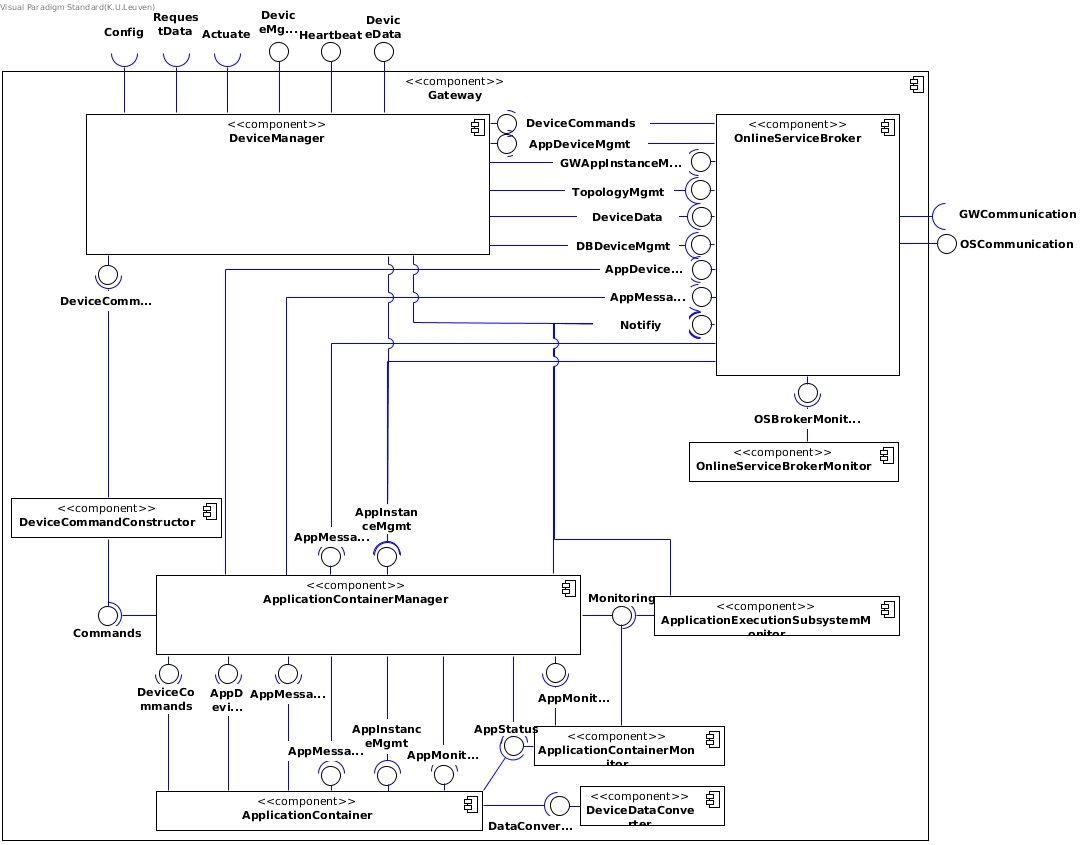
\includegraphics[width=\linewidth]{images/component-diagram-Gateway}
    	\caption[Decomposition of \texttt{Gateway}]{Decomposition of \texttt{Gateway}.\\
    	This caption contains a longer explanation over multiple lines. This additional explanation is not shown in the list of figures.}\label{fig:decomp-component1}
    \end{figure}
\end{landscape}

\begin{landscape}
    \centering
    \vspace*{\fill}

    \begin{figure}[!htp]
    	\centering
    	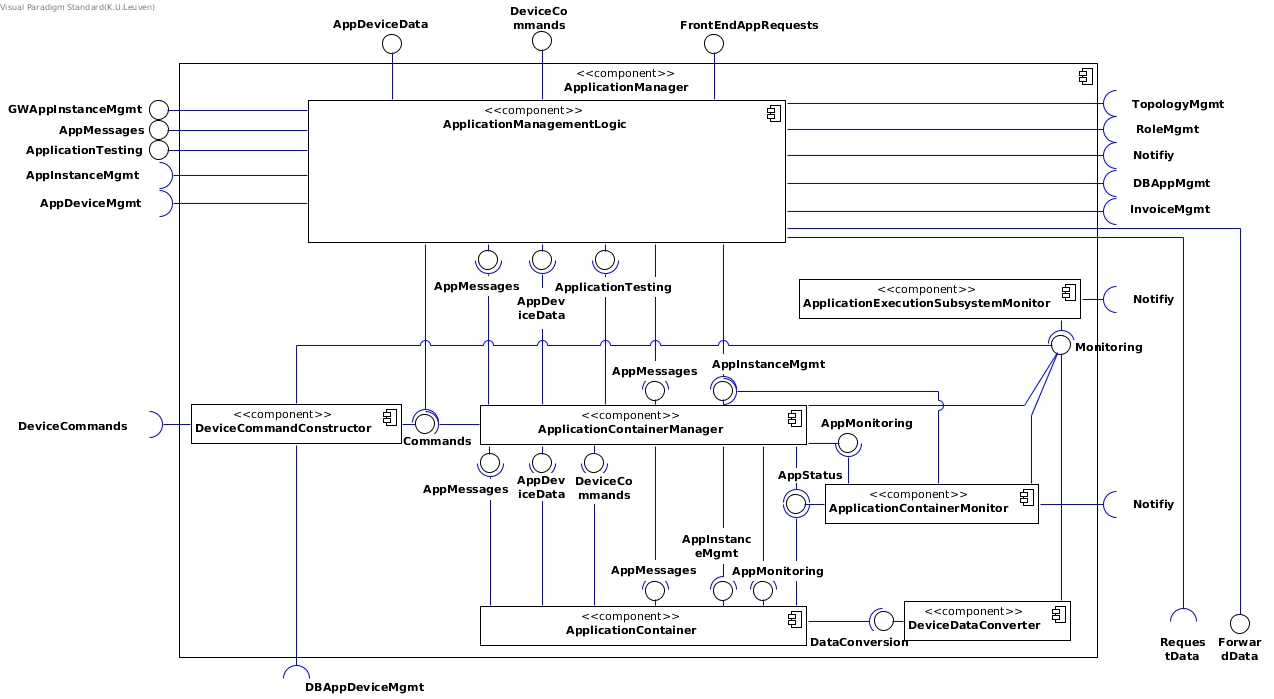
\includegraphics[width=\linewidth]{images/component-diagram-ApplicationManager}
    	\caption[Decomposition of \texttt{ApplicationManager}]{Decomposition of \texttt{ApplicationManager}.\\
    	This caption contains a longer explanation over multiple lines. This additional explanation is not shown in the list of figures.}\label{fig:decomp-component2}
    \end{figure}

    \vfill
\end{landscape}


\begin{figure}[!htp]
	\centering
	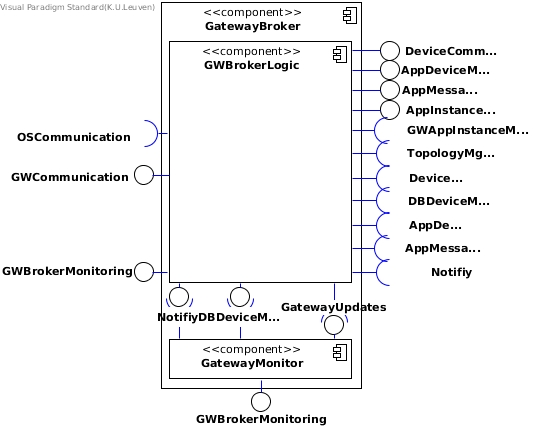
\includegraphics[width=\textwidth]{images/component-diagram-GatewayBroker}
	\caption[Decomposition of \texttt{GatewayBroker}]{Decomposition of \texttt{GatewayBroker}.\\
	This caption contains a longer explanation over multiple lines. This additional explanation is not shown in the list of figures.}\label{fig:decomp-component3}
\end{figure}


\begin{figure}[!htp]
	\centering
	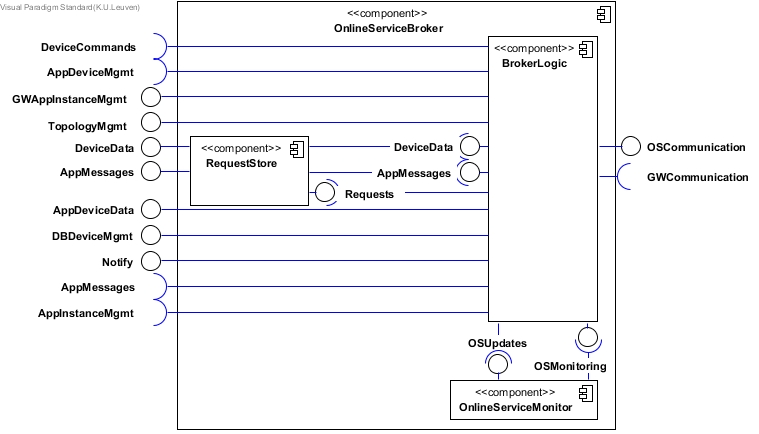
\includegraphics[width=\textwidth]{images/component-diagram-OnlineServiceBroker}
	\caption[Decomposition of \texttt{OnlineServiceBroker}]{Decomposition of \texttt{OnlineServiceBroker}.\\
	This caption contains a longer explanation over multiple lines. This additional explanation is not shown in the list of figures.}\label{fig:decomp-component4}
\end{figure}
